%%%%%%%%%%%%%%%%%%%%%%%%%%%%%%%%%%%%%%%%%
% Beamer Presentation
% LaTeX Template
% Version 1.0 (10/11/12)
%
% This template has been downloaded from:
% http://www.LaTeXTemplates.com
%
% License:
% CC BY-NC-SA 3.0 (http://creativecommons.org/licenses/by-nc-sa/3.0/)
%
%%%%%%%%%%%%%%%%%%%%%%%%%%%%%%%%%%%%%%%%%

%----------------------------------------------------------------------------------------
%	PACKAGES AND THEMES
%----------------------------------------------------------------------------------------

\documentclass{beamer}

\mode<presentation> {

% The Beamer class comes with a number of default slide themes
% which change the colors and layouts of slides. Below this is a list
% of all the themes, uncomment each in turn to see what they look like.

%\usetheme{default}
%\usetheme{AnnArbor}
%\usetheme{Antibes}
%\usetheme{Bergen}
%\usetheme{Berkeley}
%\usetheme{Berlin}
%\usetheme{Boadilla}
%\usetheme{CambridgeUS}
\usetheme{Copenhagen}
%\usetheme{Darmstadt}
%\usetheme{Dresden}
%\usetheme{Frankfurt}
%\usetheme{Goettingen}
%\usetheme{Hannover}
%\usetheme{Ilmenau}
%\usetheme{JuanLesPins}
%\usetheme{Luebeck}
%\usetheme{Madrid}
%\usetheme{Malmoe}
%\usetheme{Marburg}
%\usetheme{Montpellier}
%\usetheme{PaloAlto}
%\usetheme{Pittsburgh}
%\usetheme{Rochester}
%\usetheme{Singapore}
%\usetheme{Szeged}
%\usetheme{Warsaw}

% As well as themes, the Beamer class has a number of color themes
% for any slide theme. Uncomment each of these in turn to see how it
% changes the colors of your current slide theme.

%\usecolortheme{albatross}
%\usecolortheme{beaver}
%\usecolortheme{beetle}
%\usecolortheme{crane}
%\usecolortheme{dolphin}
%\usecolortheme{dove}
%\usecolortheme{fly}
%\usecolortheme{lily}
%\usecolortheme{orchid}
%\usecolortheme{rose}
%\usecolortheme{seagull}
%\usecolortheme{seahorse}
%\usecolortheme{whale}
%\usecolortheme{wolverine}

%\setbeamertemplate{footline} % To remove the footer line in all slides uncomment this line
%\setbeamertemplate{footline}[page number] % To replace the footer line in all slides with a simple slide count uncomment this line

%\setbeamertemplate{navigation symbols}{} % To remove the navigation symbols from the bottom of all slides uncomment this line
}

\usepackage{graphicx} % Allows including images
\usepackage{booktabs} % Allows the use of \toprule, \midrule and \bottomrule in tables
\usepackage{animate}
\usepackage{subfigure}
%----------------------------------------------------------------------------------------
%	TITLE PAGE
%----------------------------------------------------------------------------------------
\title[HiPEDS group project]{Volume estimation via integrating on a curve fitted point cloud} % The short title appears at the bottom of every slide, the full title is only on the title page

\author{\textbf{HiPEDS 2018 Cohort:} G. Bisbas, L. Castiglione, D. Grumberg, S. Karolčík, L. Keeble, D. Kulon, B. Kwan, C. McMeel, R. Miles, J. Ortiz, N. Perez-Nieves, V. Pham Ngoc, J. Vandebon, D. Vink} % Your name
\institute[Imperial College London] % Your institution as it will appear on the bottom of every slide, may be shorthand to save space
{ Imperial College London \\
	
	
	\begin{tabular}{ccc}
		
\includegraphics[width=2cm]{Figures/royalmail} &
		
\includegraphics[width=3.5cm]{Figures/epsrc} &
		
\includegraphics[width=5cm]{Figures/imperial}
	\end{tabular}

 % Your institution for the title page
\medskip % Your email address
}

\date{\today} % Date, can be changed to a custom date


\begin{document}

\begin{frame}
\titlepage % Print the title page as the first slide
\end{frame}



%% --------------T--H--E--O--R--Y-------------------------------------------

\begin{frame}
\frametitle{The problem and the goal} 
\begin{figure}	
	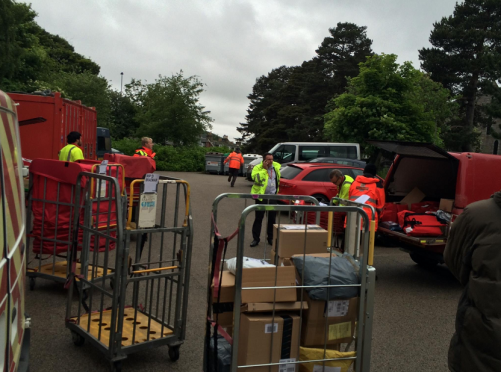
\includegraphics[width=0.5\textwidth]{Figures/royal_vans.png}
	\caption{Royal vans. \textit{Courtesy of https://www.pressandjournal.co.uk}}
	\label{vans}
\end{figure}


\begin{itemize}
	\item \textbf{Problem:} Packaging in vans is not optimal $ \rightarrow$  lots of empty space
	
	\item \textbf{Goal:} Fast estimation of available volume to ensure optimal packaging
	
\end{itemize}

\end{frame}




\begin{frame}
\frametitle{Overall structure}
\textbf{HiPEDS Group workflow}
\begin{itemize}
	\item Cohort meetings on a regular basis 
	\item Identify our goals and split into subgroups
	\item Integrate our progress
	\item Redefine goals
\end{itemize}	
\textbf{ Point cloud integration team overall checkpoints}
\begin{itemize}	

	\item Capture images
	\item Extract point cloud
	\item Fit a curve
	\item Find the volume inside
	

\end{itemize}

\textit{More details in the next slides...}

\end{frame}





%\begin{frame}
%\frametitle{The hardware - Choosing the camera fitting our needs best} % Table of contents slide, comment this block out to remove it
%\tableofcontents % Throughout your presentation, if you choose to use \section{} and \subsection{} commands, these will automatically be printed on this slide as an overview of your presentation

%Three (3) cameras were considered. Pros and cons of each were weighted and the group ended up choosing Intel RealSense D435.

%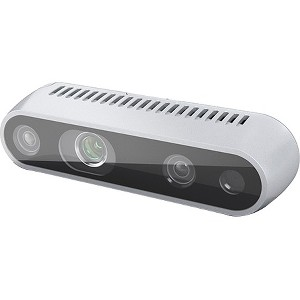
\includegraphics[width = 2cm]{Figures/Realsense1}
%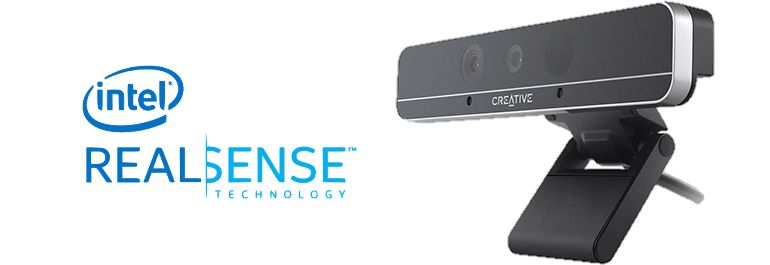
\includegraphics[width = 4cm]{Figures/intel2} \hspace{1cm}
%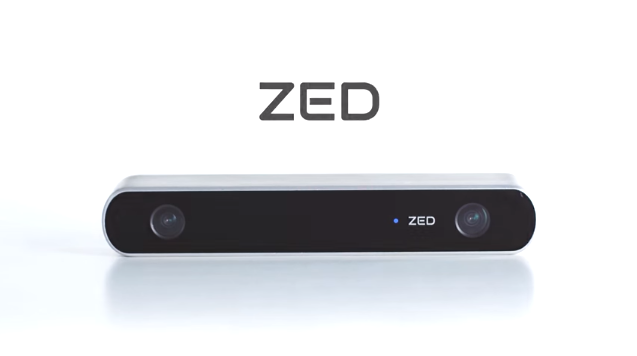
\includegraphics[width = 3cm]{Figures/ZED} \hspace{2cm}
%\\ Intel Realsense SR$300$ is better for indoor locations due to infrared light while Zed Stereo Camera is better for outdoors. Our experiments using both of them, reassured this notion. After excluding the camera that didn't work, we settled on the Realsense $D435$ due to its superior price point and lack of dependence on environmental factors.


%\begin{figure}	
%	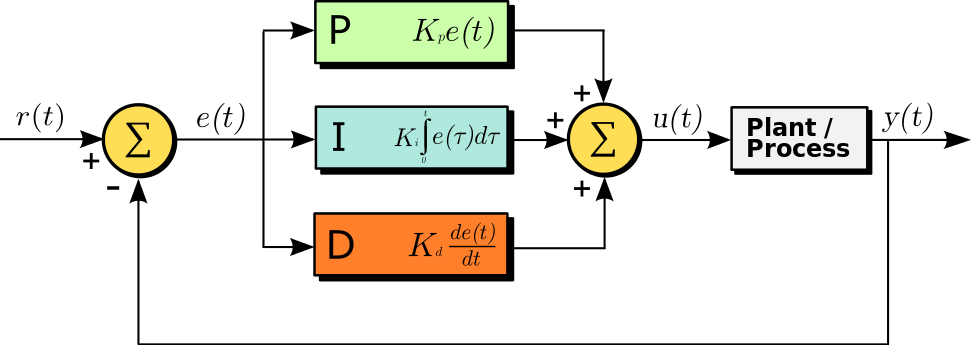
\includegraphics[width=0.8\textwidth]{Figures/PID.png}
%	\caption{PID controller}
%	\label{pid}
%\end{figure}


%\end{frame}


\begin{frame}
\frametitle{The hardware - Choosing the camera fitting our needs best} % Table of contents slide, comment this block out to remove it
%\tableofcontents % Throughout your presentation, if you choose to use \section{} and \subsection{} commands, these will automatically be printed on this slide as an overview of your presentation

% Three (3) cameras have been considered. Pros and cons of each have been weighted and the group ended up choosing Intel RealSense D435.

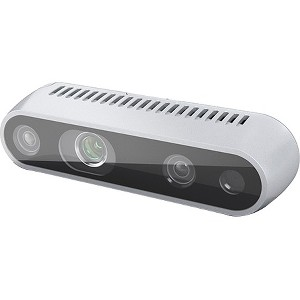
\includegraphics[width = 2cm]{Figures/Realsense1}
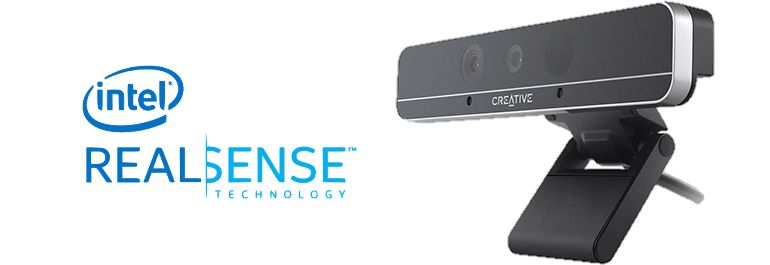
\includegraphics[width = 4cm]{Figures/intel2} \hspace{1cm}
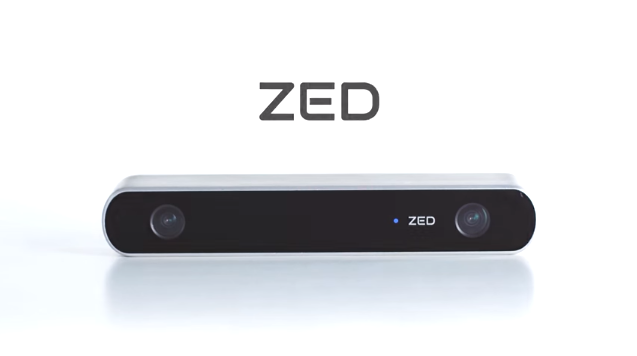
\includegraphics[width = 3cm]{Figures/ZED} \hspace{2cm}
\\ %Intel Realsense SR$300$ is better for indoor locations due to infrared light while Zed Stereo Camera is better for outdoors. Our experiments using both of them, reassured this notion. After excluding the camera that didn't work, 
The Realsense $D435$ has been proved to be the best choice.
\begin{itemize}
	\item \textbf{+ } Relatively cheap.
	
	\item \textbf{+ } Independent from lighting conditions. 
		
	\item \textbf{-} Still expensive but...
	\item \textbf{+ } ...can be used in multiple vans!	
\end{itemize}


%\begin{figure}	
%	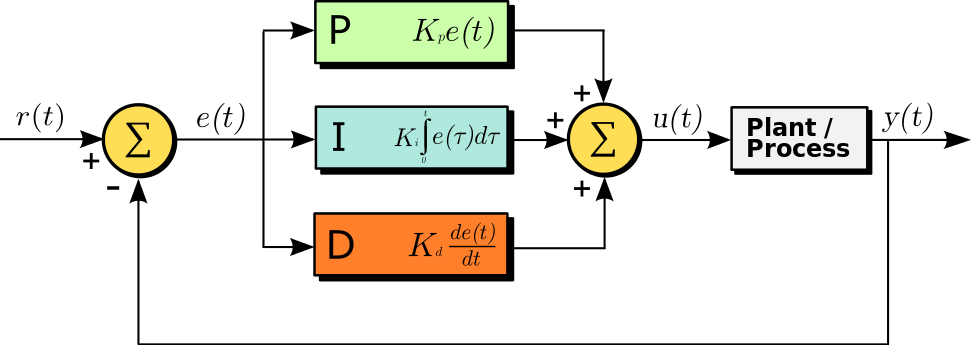
\includegraphics[width=0.8\textwidth]{Figures/PID.png}
%	\caption{PID controller}
%	\label{pid}
%\end{figure}


\end{frame}
%\subsection{Subsection Example} % A subsection can be created just before a set of slides with a common theme to further break down your presentation into chunks

\begin{frame}\frametitle{Extracting the point cloud: PLYExtractor}

Using the RealSense SDK, a piece of software has been written to automatise the process of extracting pointclouds from different points of view 

\begin{figure}	
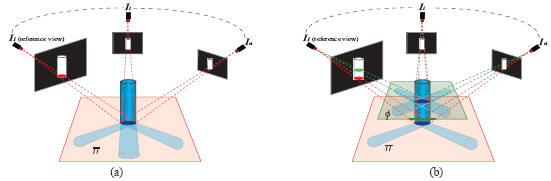
\includegraphics[width=0.8\textwidth]{Figures/Resear10.jpg}
% \caption{Software Activity Flow}
\label{fig:Reco}
\end{figure}

\end{frame}

\begin{frame}\frametitle{PLYExtractor: Activity Flow}

\begin{figure}	
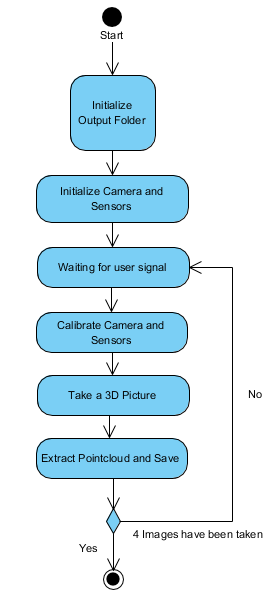
\includegraphics[width=0.27\textwidth]{Figures/ActvityFlow.PNG}
\caption{Software Activity Flow}
\label{fig:ActivityFlow}
\end{figure}


\end{frame}

\begin{frame}\frametitle{PLYExtractor: in Action}

\begin{figure}
\hfill
\subfigure[ ]{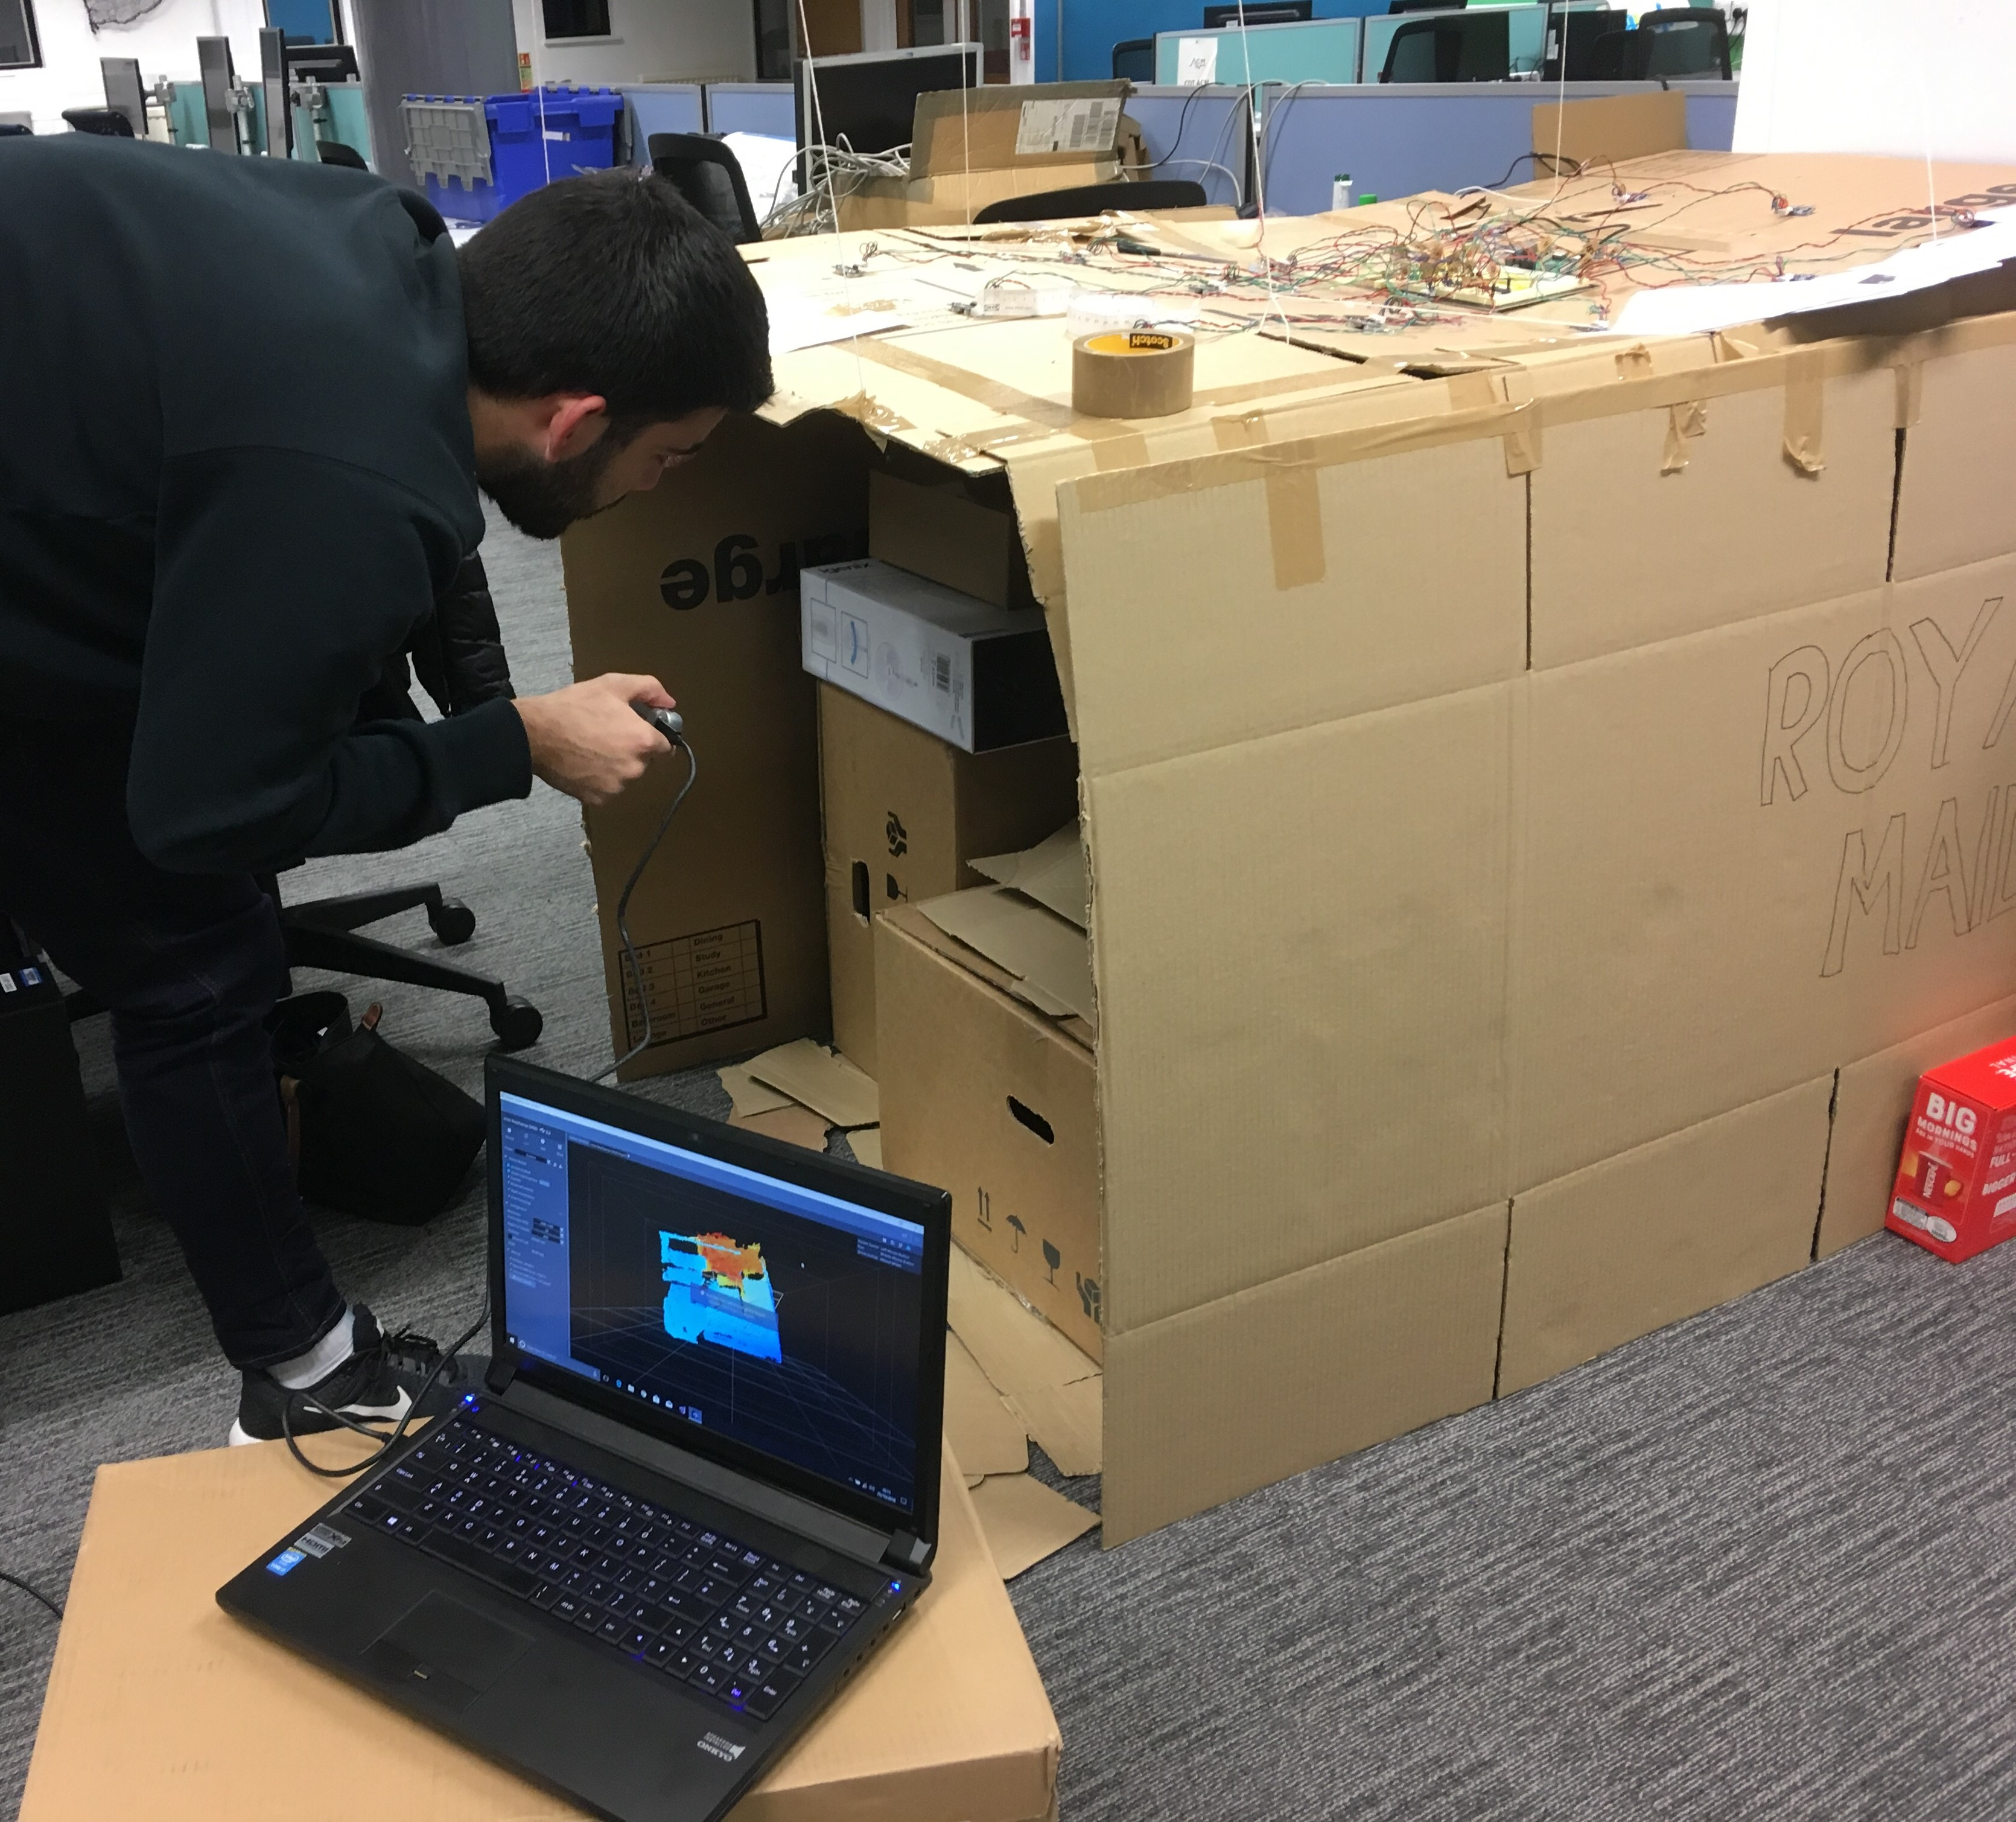
\includegraphics[width=5cm]{Figures/action2.jpg}}
\hfill
\subfigure[ ]{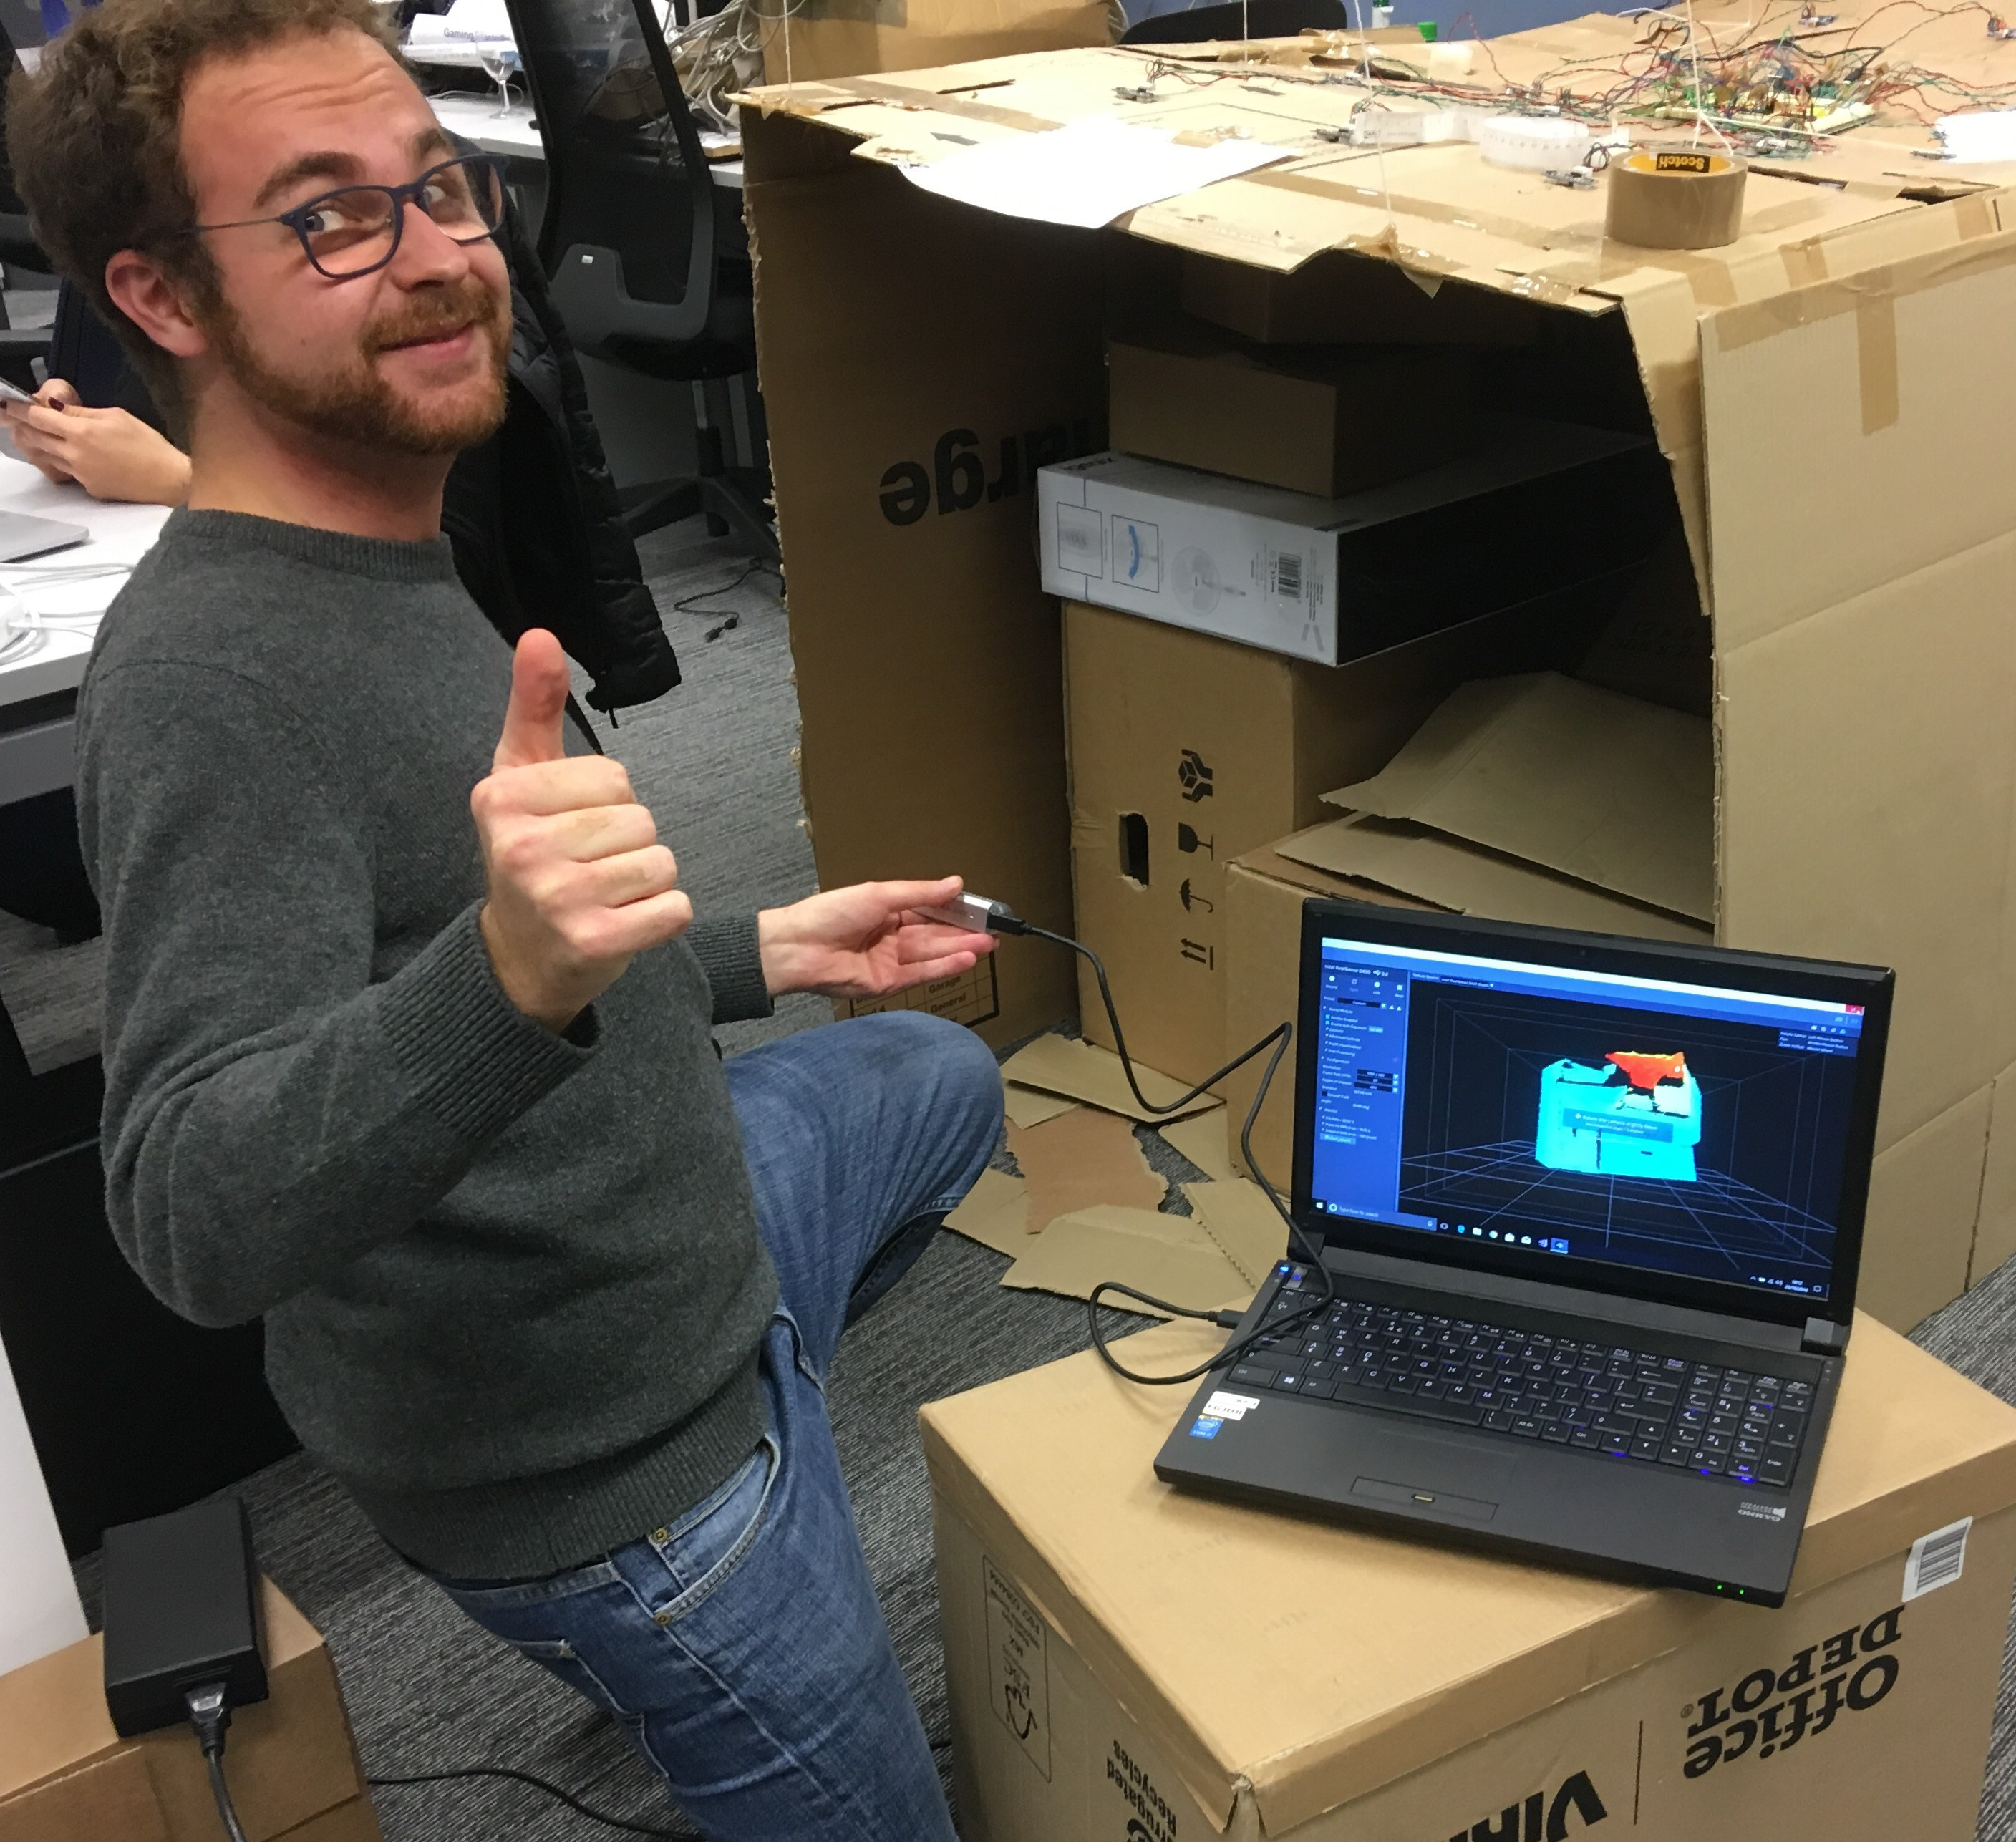
\includegraphics[width=5cm]{Figures/action1.jpg}}
\hfill
\end{figure}


\end{frame}


%\subsection{Subsection Example} % A subsection can be created just before a set of slides with a common theme to further break down your presentation into chunks


\begin{frame}{Denoising the point cloud}
Extracted point clouds are often very noisy, so, a need for removing outliers is needed.

\begin{itemize}
	\item Step 1: Hard-cut denoising of points that are very far away of the mass centre.
	\item Step 2: Use a nearest neighbours approach with a predefined threshold to remove more outliers. 
\end{itemize}

Resulted point clouds were found to be \textbf{95\%} correctly denoised via simple parameter tuning.
\begin{figure}
	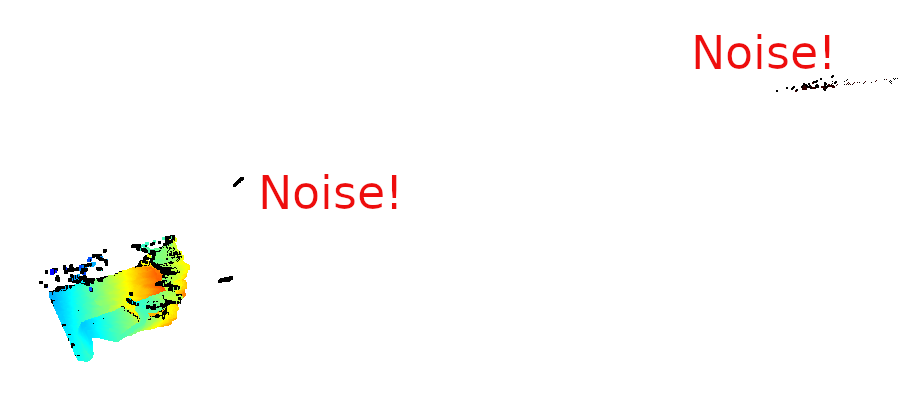
\includegraphics[width=0.6\linewidth]{Figures/noisy}
	\label{noisy}
	\caption{A noisy point cloud.}
\end{figure} 


\end{frame}

%----------------------------------------------------------------------
\begin{frame}{The ICP algorithm}

{\small The Iterative Closest Points algorithm was used to merge the different point clouds extracted from the camera.

For each point in the source point cloud, match the closest point in the reference point cloud (or a selected set).
\begin{enumerate}
	\item Estimate the combination of rotation and translation using a root mean square point to point distance metric minimization technique which will best align each source point to its match found in the previous step. This step may also involve weighting points and rejecting outliers prior to alignment.
	\item Transform the source points using the obtained transformation.
	\item Iterate (re-associate the points, and so on).
\end{enumerate}}
\end{frame}

%----------------------------------------------------------------------

\begin{frame}{Merging point clouds}

\begin{columns}
	\begin{column}{0.5\textwidth}
	%	\begin{center}
\textbf{Merging procedure:} 2 steps\\

1st  step: 4 to 2\\
2nd step: 2 to 1\\

\begin{figure}
	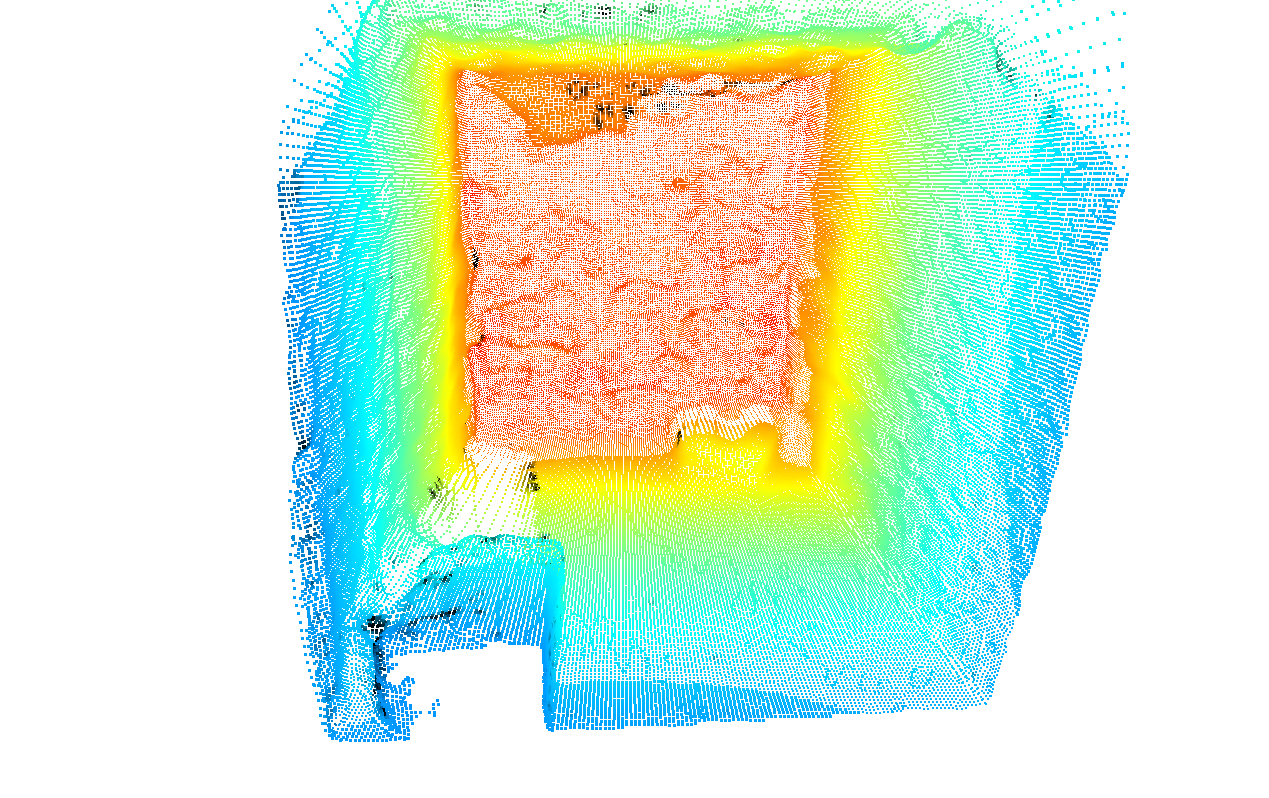
\includegraphics[width=0.8\linewidth]{Figures/depth02.png}
	\label{depth02}
	\caption{ After merging.}
\end{figure}

	%	\end{center}
	\end{column}
	\begin{column}{0.6\textwidth}  %%<--- here
		\begin{center}
			\begin{figure}
				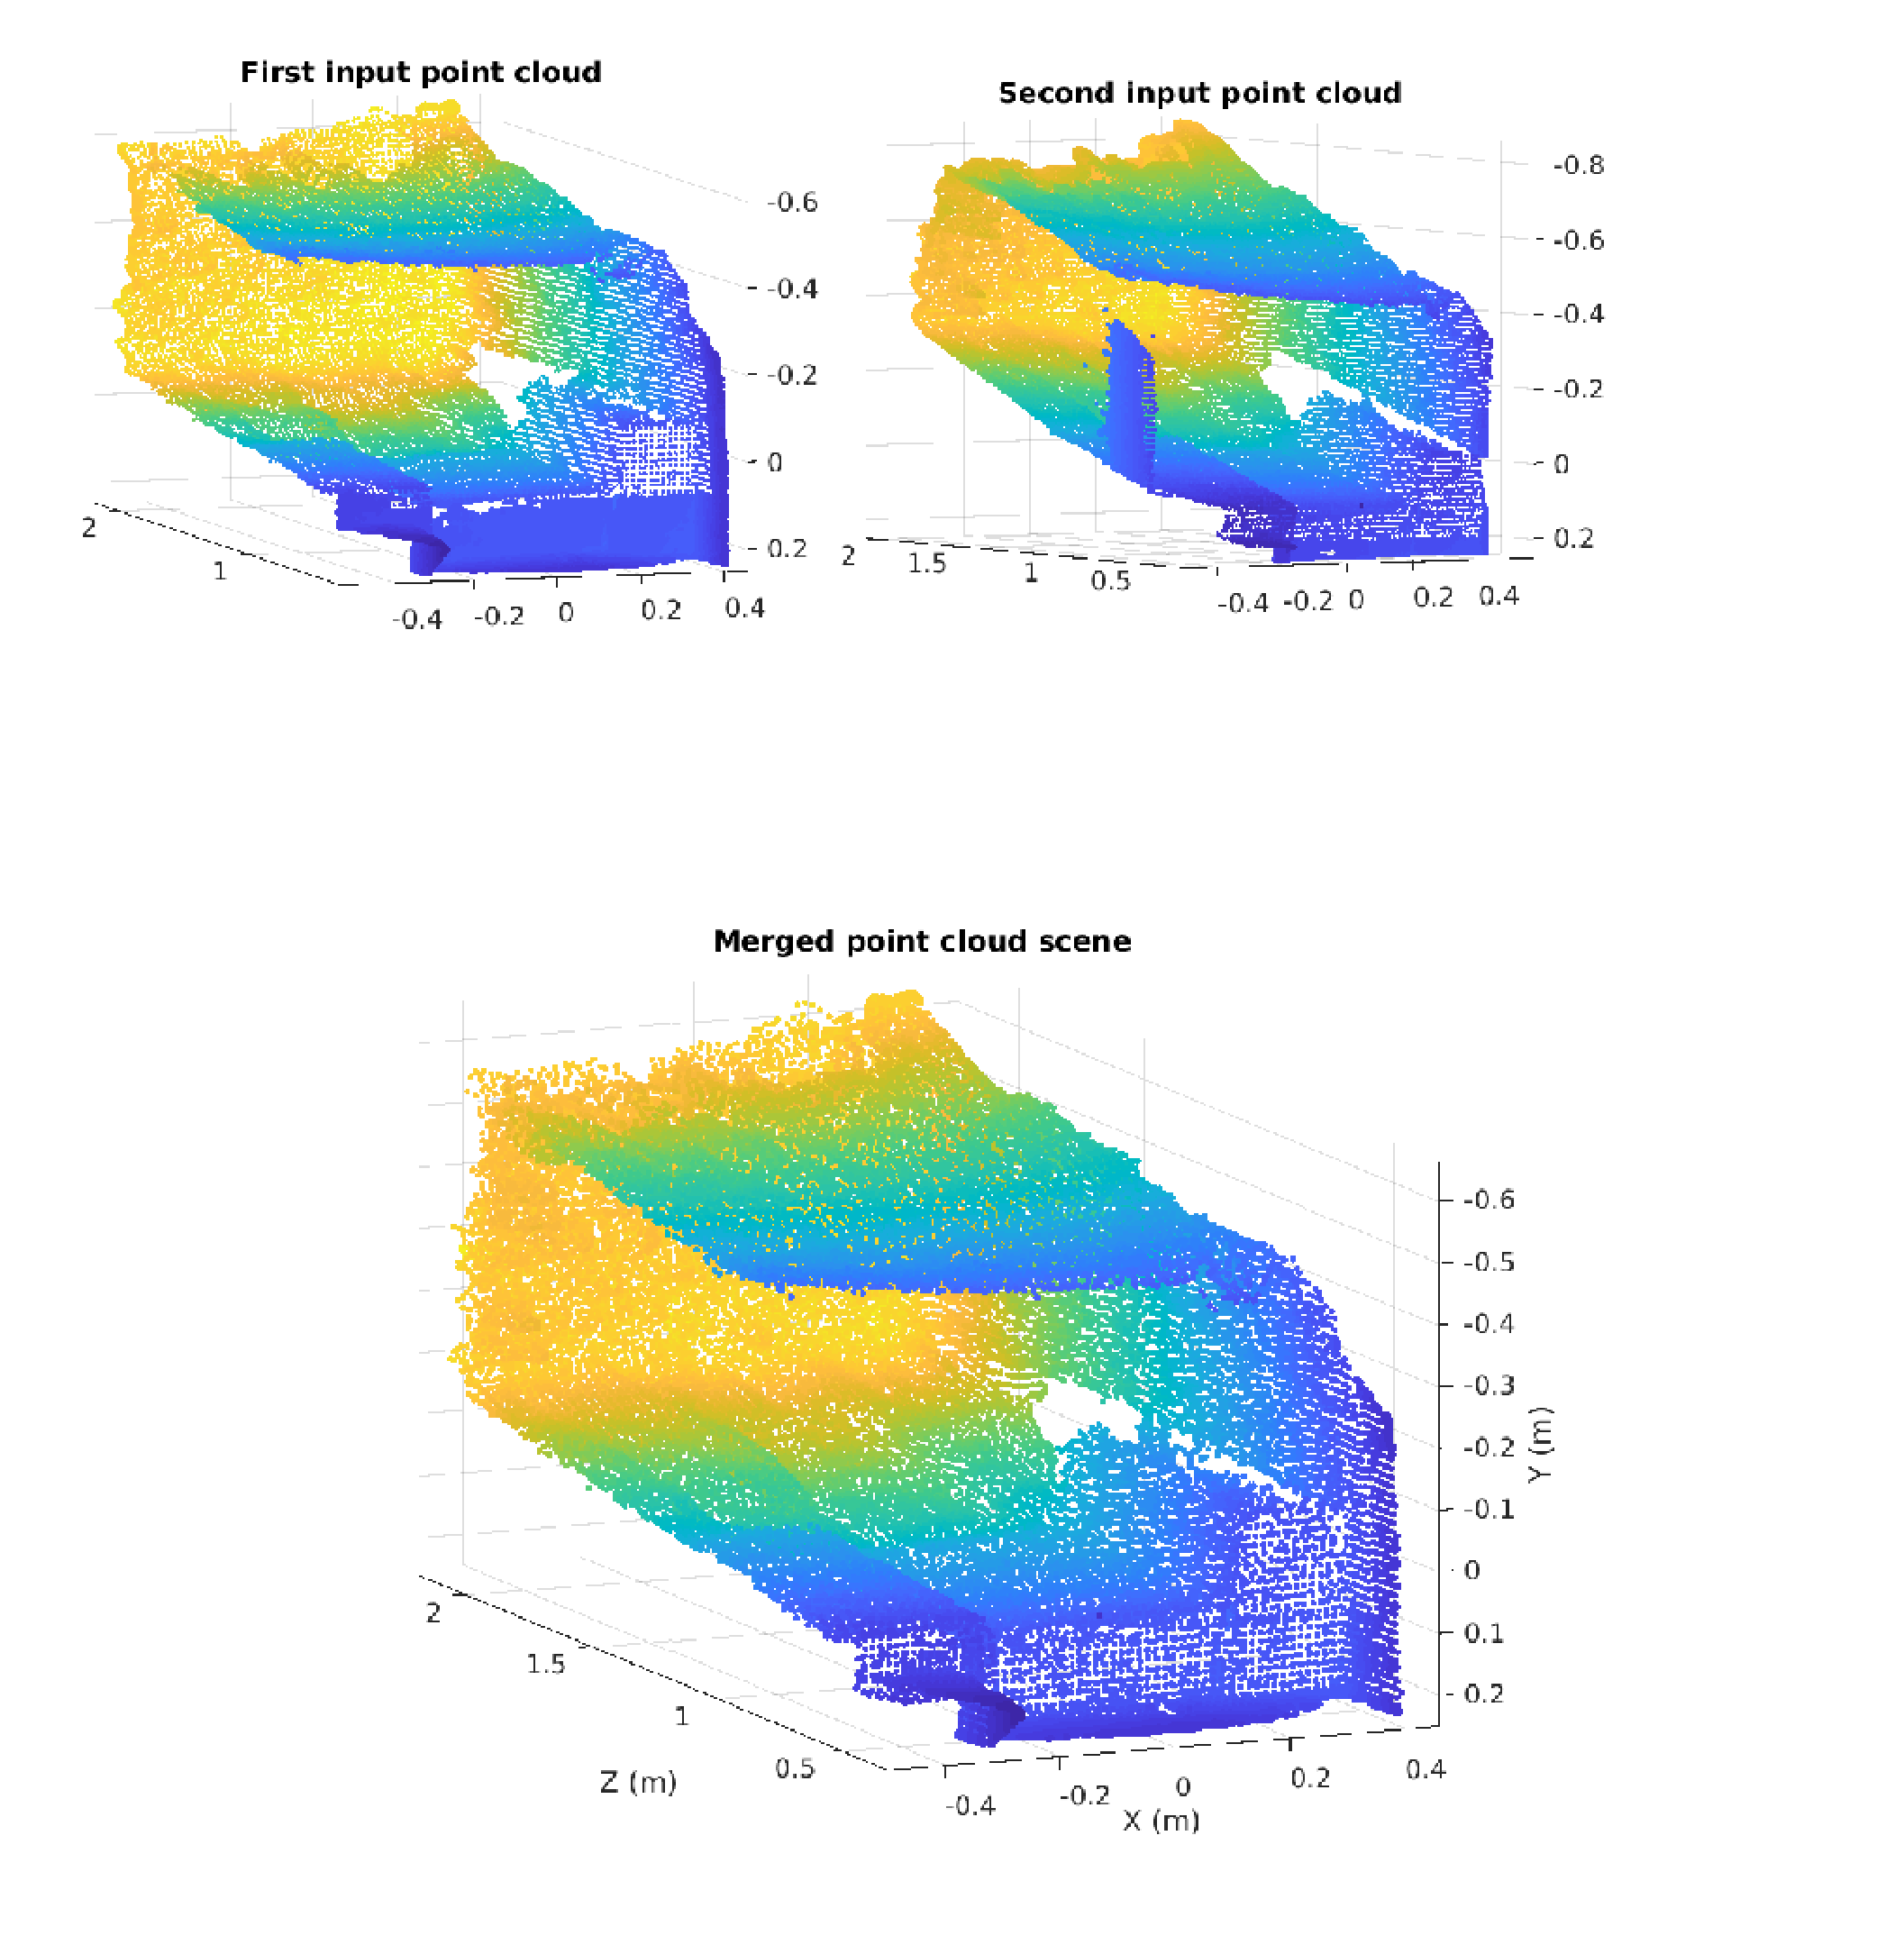
\includegraphics[width=0.8\linewidth]{Figures/merge_h.eps}
				\label{merge}
				\caption{ Intermediate merged pointclouds (left) and final point cloud (right). Denoised and downsampled version of final point cloud (bottom).}
			\end{figure}

		\end{center}
	\end{column}
\end{columns}


\end{frame}
%----------------------------------------------------------------------


\begin{frame}{Curve fitting with Linear Interpolation}

\begin{columns}
	\begin{column}{0.49\textwidth}
		%\begin{left}
Using MATLAB's Curve Fitting Toolbox, we managed to 
\begin{itemize}
	\item Fit a polynomial surface
	\item Step 2: Use a nearest neighbours approach with a predefined threshold to remove more outliers. 
\end{itemize}

Resulted point clouds were found to be \textbf{95\%} correctly denoised via simple parameter tuning.
		%\end{left}
	\end{column}
	\begin{column}{0.6\textwidth}  %%<--- here
		\begin{center}
			\begin{figure}
				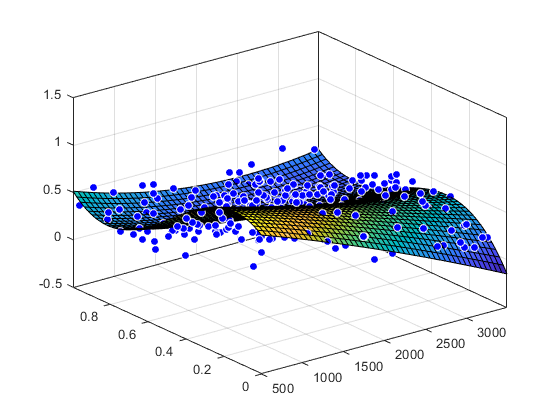
\includegraphics[width=0.6\linewidth]{Figures/FitA}
				\label{fitA}
				\caption{A simple curve fitting}
			\end{figure}
			\begin{figure}
				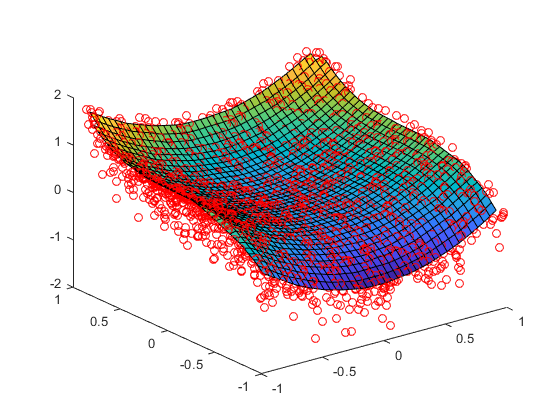
\includegraphics[width=0.5\linewidth]{Figures/interp}
				\label{interp}
				\caption{Linear interpolation}
			\end{figure}
			
		\end{center}
	\end{column}
\end{columns}

\end{frame}

%----------------------------------------------------------------------

\begin{frame}{Integration -  Keep it simple scientist}
\begin{columns}
\begin{column}{0.5\textwidth}  %%<--- here
	\begin{center}
	\begin{equation}
	\iiint_V f(x,y,z) \,dx\,dy\,dz 
	\end{equation}
	
	\animategraphics[loop,controls,width=0.7\linewidth]{4}{Figures/gif/sweep-}{0}{32}
		
	
	%\begin{figure}
	%	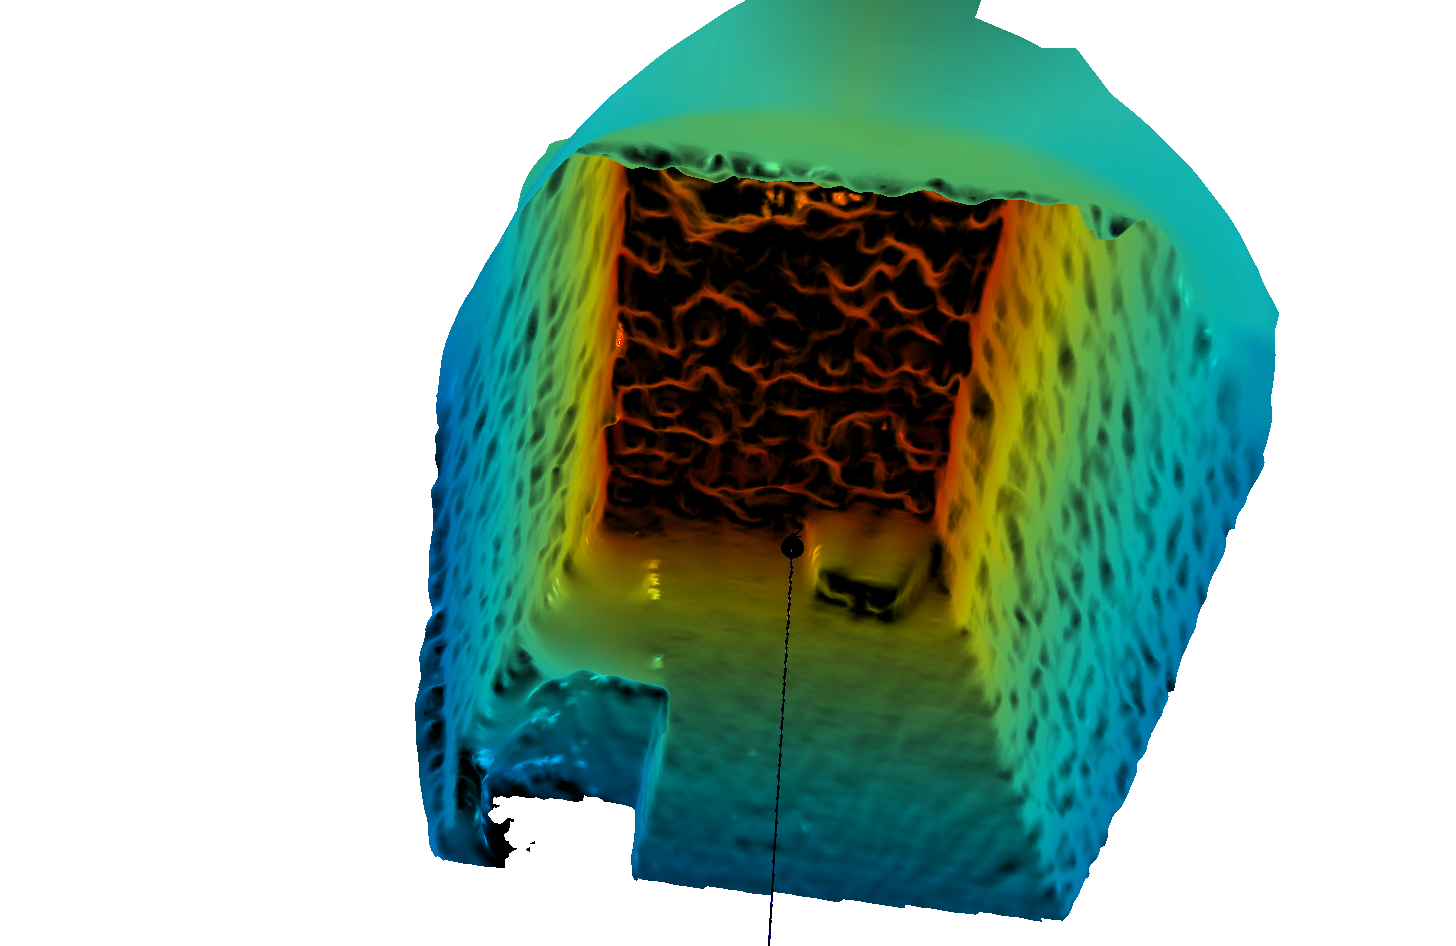
\includegraphics[width=0.5\linewidth]{Figures/meshlab}
	%	\label{meshlab1}
	%	\caption{A full fitted surface}
	%\end{figure}
	\end{center}
\end{column}
\begin{column}{0.5\textwidth}  %%<--- here
	\begin{center}
	%	\begin{equation}
	%	\iiint_V f(x,y,z) \,dx\,dy\,dz 
	%	\end{equation}
\begin{figure}
	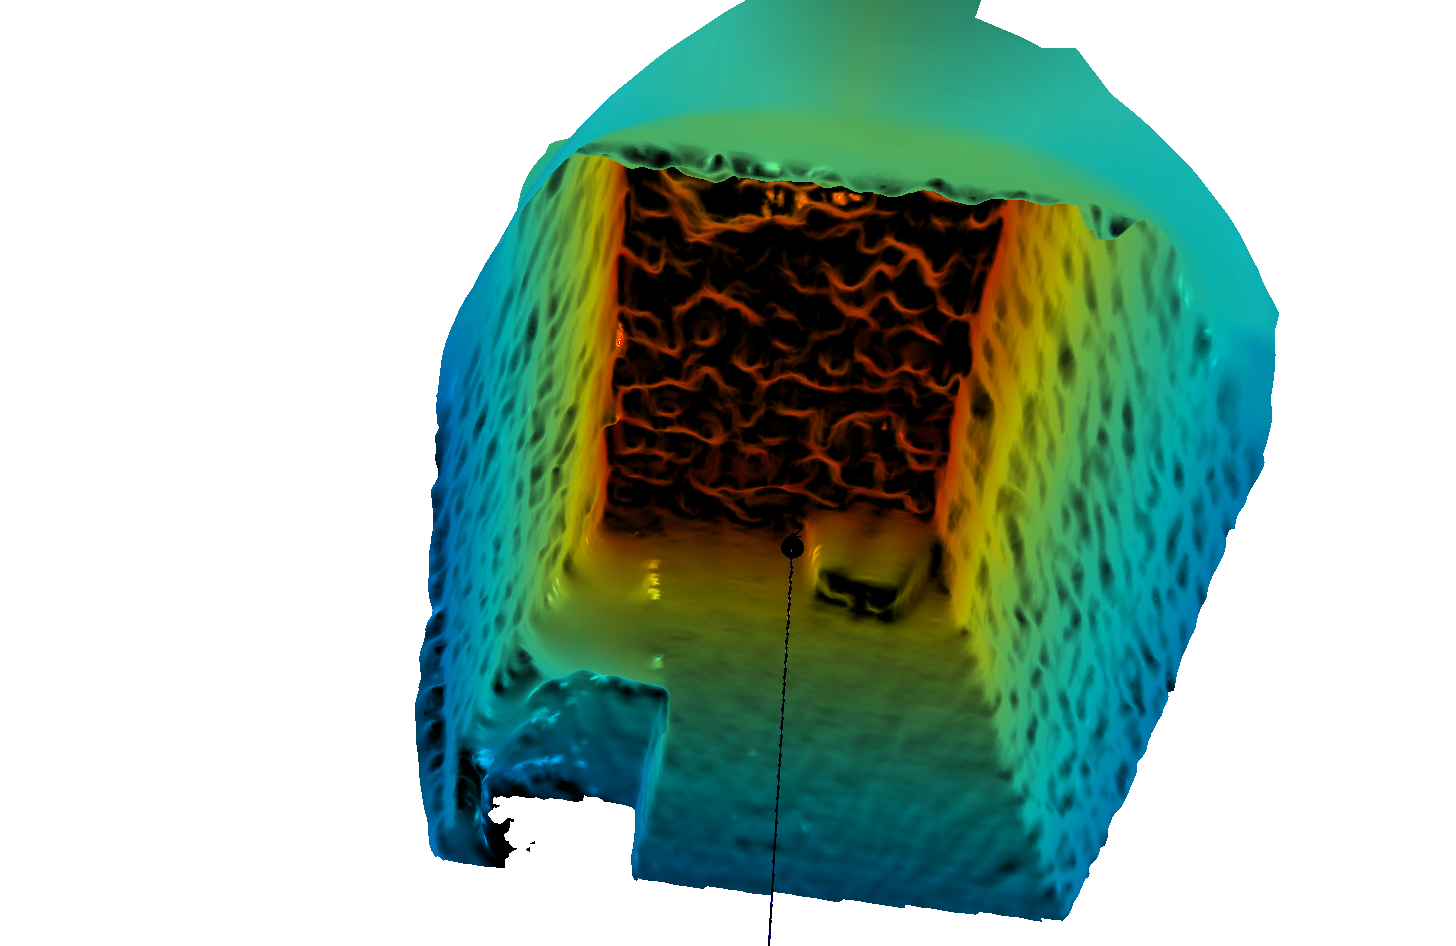
\includegraphics[width=0.75\linewidth]{Figures/meshlab}
	\label{meshlab2}
	\caption{A full curve fitted surface}
\end{figure}

		\begin{figure}
			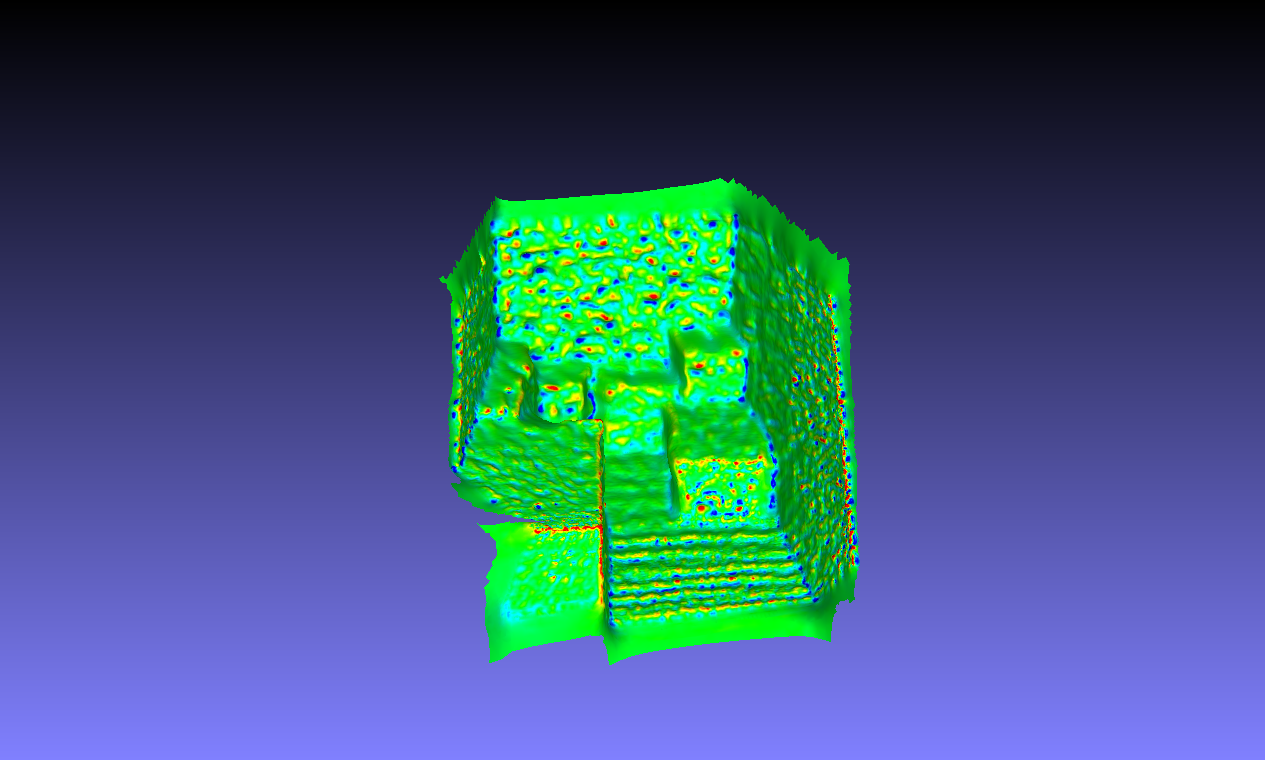
\includegraphics[width=0.75\linewidth]{Figures/curvature00}
			\label{curv}
			\caption{Curvature of the surface}
		\end{figure}
	\end{center}
\end{column}
\end{columns}



\end{frame}

%----------------------------------------------------------------------
\begin{frame}{Results-1}

\begin{figure}
	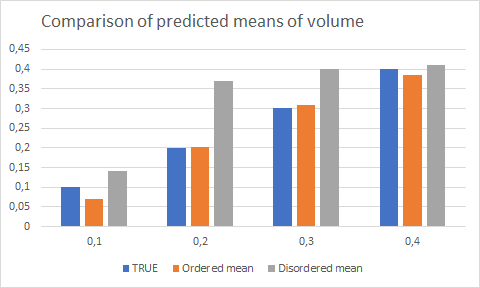
\includegraphics[width=0.95\linewidth]{Figures/chart1}
	\label{ch1}
	\caption{Comparison of ordered and disordered setups with the real occupied volume}
\end{figure}
\end{frame}


\begin{frame}{Results-2}
\begin{figure}
	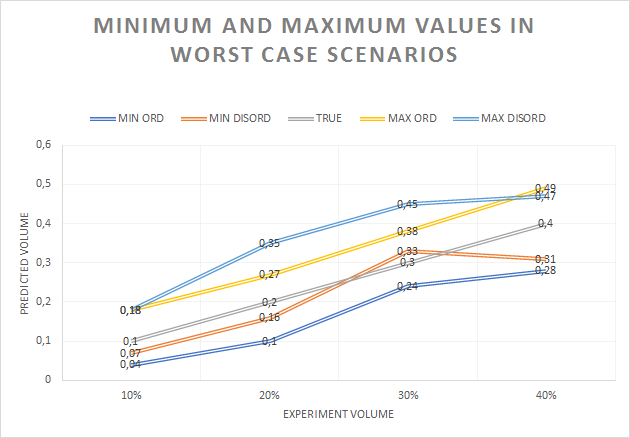
\includegraphics[width=0.9\linewidth]{Figures/chart2}
	\label{ch2}
	\caption{Worst case scenario differences}
\end{figure}
\end{frame}

\begin{frame}{Conclusion-Our proposal}
\begin{itemize}
	\item 1 camera needs 10 seconds in every van - Up to 6 vans per minute sequentially.
	\item Occupied volume prediction in less than 45 seconds for every van.
	\item 3\% - 4\% error in 85\% of cases - Worst case scenario errors up to 11\%.
	\item With less than 200gbp we should be able to calculate the volume of 100 vans in less than 20 minutes, a second camera ... 200 vans...etc...
	\item Not real time but requirements met.
	\item Simplicity - No installments
	\item Only external use
	\item Easy to transfer hardware
	\item Solution ready to be tested as soon as possible
\end{itemize}



\end{frame}

\begin{frame}{Things to consider}

\begin{itemize}
	\item Time limitations
	\item Manual Procedure
	\item Free software to reduce cost?
\end{itemize}
\end{frame}

\begin{frame}{Future extensions}

\begin{itemize}
	\item Depth picture quality
	\item Faster calculations
	\item Camera price trends
\end{itemize}
\end{frame}



%----------------------------------------------------------------------


\begin{frame}{References}
\begin{enumerate}
	\item Z. Zhang, “Iterative point matching for registration of free-form curves and surfaces,” Int. J. Comput. Vis., 1994.
	\item E. Johnson and M. Hebert, “Surface registration by matching oriented points,” Proceedings. Int. Conf. Recent Adv. 3-D Digit. Imaging Model. (Cat. No.97TB100134), 1997.
	\item  P. Besl and N. McKay, “A Method for Registration of 3-D Shapes,” Tpami, 1992.
	\item M. Kazhdan and H. Hoppe, “Screened poisson surface reconstruction,” ACM Trans. Graph., vol. 32, no. 3, pp. 1–13, 2013.
	\item N. Amenta, S. Choi, and R. K. Kolluri, “The power crust,” Proc. sixth ACM Symp. Solid Model. Appl. - SMA ’01, pp. 249–266, 2001.
	\item M. Kazhdan, M. Bolitho, and H. Hoppe, “Poisson Surface Reconstruction,” Proc. Symp. Geom. Process., pp. 61–70, 2006.
\end{enumerate}
\end{frame}

%------------------------------------------------

%------------------------------------------------


%------------------------------------------------

\begin{frame}{Acknowledgements}
This project was proposed and supported by Royal Mail, EPSRC and Imperial College London. We would like to than all the HiPEDS 1st year PhD students for their cooperation and a special thanks to Jeremy Bradley and Ben Glocker for their support and advice throughout.\\
	\begin{tabular}{ccc}
	
\includegraphics[width=2cm]{Figures/royalmail} &
	
\includegraphics[width=3.5cm]{Figures/epsrc} &
	
\includegraphics[width=5cm]{Figures/imperial}
\end{tabular}
\end{frame}

%----------------------------------------------------------------------------------------

\end{document}